\documentclass[nobib]{MSword}
% Class options:
%-------------------------------
% nobib         - skip bibliography code/ don't include bib
% math          - include math packages and useful math commands
% hidelinks     - hide hyperref colored link boxes
% wordlinks     - link color scheme similar to word


% Preamble code:
%%%%%%%%%%%%%%%%%%%%%%%%%%%%%%%%%%%%%%%%
\usepackage[spanish]{babel}
\usepackage{csquotes}
\usepackage{parskip}

% % Uncomment using "Ctrl + /" (/ on numpad):
% % Customizing headers and footers:
% \fancypagestyle{custom}{%
%     \fancyhf{}% clears the footer and header
%     % Header:
%     \fancyhead[L]{}
%     \fancyhead[C]{}
%     \fancyhead[R]{}
%     % Footer:
%     \fancyfoot[L]{}
%     \fancyfoot[C]{}
%     \fancyfoot[R]{}
%         % Tips:
%         % ----
%         % L: left, C: center, R: right
%         % O: odd pages, E: even pages
%         % ----
%         % Example: \fancyghead[LO,RE]{Text}
%         % will produce "Text" left in the header
%         % on odd pages and right in the header on even pages.
%     % Rules/ lines:
%     \renewcommand{\headrulewidth}{0.4pt}
%     \renewcommand{\footrulewidth}{2pt}
% }
% % Changing the pagestyle:
% \pagestyle{custom}

%%%%%%%%%%%%%%%%%%%%%%%%%%%%%%%%%%%%%%%%

% Preamble information:
%%%%%%%%%%%%%%%%%%%%%%%%%%%%%%%%%%%%%%%%

\title{Documentacion}
\author{Aldo Javier Ángeles Sánchez\\ Arlet Pinacho Báez \\
  Juvenal Guzmán Condado \\ Ricardo Iván Martínez Cano \\
  Ricardo Maximiliano Victoria Morales \\ Monserrat Mendez Camacho}
\date{25/03/25}

%%%%%%%%%%%%%%%%%%%%%%%%%%%%%%%%%%%%%%%%

% The document:
%%%%%%%%%%%%%%%%%%%%%%%%%%%%%%%%%%%%%%%%
\begin{document}

\maketitle

\section{Introduccion}
% Text files from txt folder:
El objetivo de este documento es proporcionar una vista general para el desarrollo de un sistema destinado a la gestión de incidentes urbanos. Se abordarán los aspectos clave para el desarrollo de dicho sistema, como los requerimientos funcionales y no funcionales,  el diseño de la arquitectura y las fases del desarrollo.

Durante el desarrollo del proyecto se busca llevar a cabo un método incremental que permita entregar en cada fase resultados parciales que puedan ser validados por el cliente.

\subsection{Propósito del sistema.}

Se busca desarrollar una página web para el registro y gestión de incidentes urbanos por medio de la participación activa de los ciudadanos. Esto con el fin de a largo plazo hacer uso de los datos recopilados para la optimización de la resolución y seguimiento brindado por las autoridades gubernamentales.

\subsection{Alcance del sistema.}

Dado que el proyecto busca fomentar la participación de la ciudadanía, la funcionalidad prioritaria será permitir a los usuarios (ciudadanos de la CDMX) registrarse en la plataforma web, lo que les habilitará para crear, actualizar y visualizar incidentes relacionados con la vía pública. Los registros de incidentes incluirán información esencial como la ubicación y una descripción del problema, permitiendo un seguimiento adecuado.

\subsection{Definiciones y abreviaciones.}
\begin{itemize}
    \item Salting: Técnica criptográfica que consiste en añadir un valor aleatorio único (llamado salt) a cada contraseña antes de calcular su hash. 
    \item Hashing: Forma de cifrar las contraseñas a través de una función hash criptográfica. Esto para tener más seguridad.
    \item Estado de un accidente: Puede ser "Reportado", "En proceso" o "Resuelto". Se refiere a etiquetas asociadas a los accidentes registrados.
    \item MojarraDrive: Nombre de la página web a implementar.
\end{itemize}

\section{Analisis de requerimientos}
\subsection{Requerimientos del Sistema}
\subsection{Requerimientos funcionales}
\begin{itemize}
    \item Creación de cuentas para los usuarios de la página.
    
    El sistema debe permitir a cada nuevo usuario crear una cuenta que lo identifique como ciudadano y resguardar su información para posteriores ingresos a la plataforma. 
    
    \item Registro de incidentes.
    
    Se debe permitir a los usuarios llevar un registro de los incidentes que reportan. Cada incidente deberá incluir la ubicación, al menos una fotografía, un estado (Reportado, En proceso, Resuelto) y una descripción. Además, por cuestiones de administración de la información, se debe contar con una forma de clasificar los incidentes y poder identificar al usuario que los reporta.
    
    \item Clasificación de incidentes.
    
    Además de tener asociado un estado (Reportado, En proceso, Resuelto), cada incidente debe clasificarse por tipo (por ejemplo: bache, luminaria descompuesta, obstáculo en vía pública, entre otros).
    
    \item Actualización del estado de los incidentes.
    
    Es importante que el sistema permita a los usuarios actualizar el estado de los incidentes (aunque no hayan sido ellos quienes los registraron), siempre y cuando adjunten al menos una fotografía que respalde el cambio de estado.
    
    \item Visualización y filtrado de incidentes.
    
    La página debe permitir a los usuarios marcar la ubicación de los incidentes que reportan en un mapa interactivo. Además, todos los usuarios deben poder ver los incidentes reportados en la página y filtrarlos por tipo y estado.

\end{itemize}

\subsection{Requerimientos no funcionales}
\begin{itemize}
    \item Delimitación de roles\\
    El sistema no debe de permitir a un usuario que no cuenta con los permisos necesarios realizar operaciones que solo usuarios privilegiados (Administradores, Etc.) puedan realizar.
    \item Delimitación de usuarios\\
    El sistema no puede permitir que un usuario que no es el dueño de un reporte pueda realizar acciones como la eliminación del reporte, cambio de ubicación de este, cambio de descripción del reporte, cambio de clasificación del incidente.
    \item Inicio de sesión seguro\\
    El sistema debe de usar tecnología de inicio de sesión segura, ya sea utilizar un sistema de inicio de sesión popular (Inicio de sesión con cuenta de Google, Facebook) o bien utilizar un sistema de inicio de sesión desarrollado propiamente. El cuál no permita el acceso a cuentas no registradas, no permita duplicidad de cuentas, es decir, una sola cuenta puede estar asociada solo con un correo electrónico. Por último el sistema debe de ser capaz de solo aceptar correos electrónicos válidos.
    \item Contraseñas seguras\\
    Al momento de hacer el registro de un nuevo usuario, el sistema debe de revisar si la contraseña introducida por el usuario cuenta con la mínima seguridad indispensable (Por lo menos una letra mayúscula, Un caracter especial, Por lo menos un número, etc). En caso de no contar con esta información, se debe de indicar al usuario que debe de corregir antes de poder registrar a su cuenta.
    \item Validación de campos\\
    El sistema debe de validar los campos que el usuario debe de introducir para evitar situaciones de seguridad como la inyección de código.
    \item Protección de contraseñas\\
    Las contraseñas de usuario deben de estar guardadas con un estándar de cifrado usado comúnmente y seguro, de la misma manera se debe de usar un proceso de ''salting" para proveer más seguridad a los usuarios.
\end{itemize}

%\subsection{Requerimientos de dominio}

\subsection{Casos de Uso}
%Me rifo esto 

\textbf{\large CU1: Registrar un Incidente} \\

\textbf{Actores:} Usuario \\

\textbf{Flujo Principal:}
\begin{enumerate}
    \item El usuario inicia sesión en la aplicación web \texttt{MojarraDrive}.
    \item Selecciona la opción "Reportar incidente".
    \item Ingresa la ubicación del incidente en el mapa interactivo.
    \item Adjunta una o más fotografías del incidente.
    \item Clasifica el incidente según sus características
    \item Escribe una breve descripción del incidente.
    \item Confirma el registro del incidente.
    \item El sistema guarda y verifica la información.
    \item Una vez se haya confirmado la validez del incidente se muestra en el mapa de la aplicación.
\end{enumerate}

\textbf{Flujo Alternativo:}
\begin{itemize}
    \item Si se detecta algún error en la información o falta información obligatoria, el sistema notificará al usuario y solicitará completar o corregir los campos faltantes. De no completarlo correctamente, el incidente no se mostrará en el mapa. 
\end{itemize}

\vspace{0.5cm}

\textbf{\large CU2: Actualizar Estado de un Incidente} \\

\textbf{Actores:} Usuario \\

\textbf{Flujo Principal:}
\begin{enumerate}
    \item El usuario inicia sesión en la aplicación web \texttt{MojarraDrive}.
    \item Busca un incidente en el mapa o en la lista de reportes.
    \item Selecciona el incidente y elige la opción "Actualizar estado".
    \item Agrega el nuevo estado del incidente.
    \item Adjunta evidencia fotográfica del nuevo estado del incidente.
    \item Confirma la actualización del estado.
    \item El sistema cambia el estado del incidente y almacena el historial de modificaciones.
\end{enumerate}

\textbf{Flujo Alternativo:}
\begin{itemize}
    \item Si el usuario no adjunta pruebas fotográficas, el sistema rechazará la actualización del estado.
\end{itemize}

\vspace{0.5cm}

\textbf{\large CU3: Visualizar Incidentes} \\

\textbf{Actores:} Usuario \\

\textbf{Flujo Principal:}
\begin{enumerate}
    \item El usuario accede a la aplicación web \texttt{MojarraDrive}.
    \item Visualiza un mapa interactivo con incidentes reportados.
    \item Aplica filtros por tipo de incidente, estado y lugar.
    \item Selecciona un incidente para ver detalles y fotografías adjuntas.
\end{enumerate}

\vspace{0.5cm}

\textbf{\large CU4: Administración de Incidentes} \\

\textbf{Actores:} Administrador \\

\textbf{Flujo Principal:}
\begin{enumerate}
    \item El administrador inicia sesión en la aplicación web
    \texttt{MojarraDrive}.
    \item Accede al panel de administración.
    \item Filtra incidentes por tipo o estado.
    \item Modifica, elimina o marca incidentes como revisados.
    \item Genera estadísticas sobre incidentes registrados.
\end{enumerate}


\subsubsection{Casos de uso de Usuarios}
\subsection{Casos de uso del usuario}
El usuario realiza varios casos de uso en el sistema, tales como registro, inicio de sesión y actualización de credenciales. A continuación, se muestra el flujo de cada uno de los casos de uso del usuario, incluyendo los casos normales, alternativos y excepcionales. Además, se agregan diagramas que ejemplifican los flujos de dichos casos de uso.

\textbf{\large CU1: Registro en el sistema} \

\textbf{Actores:} Usuario, Sistema \

\textbf{Flujo Normal de eventos:}
\begin{enumerate}
\item El usuario accede a la página de inicio de la aplicación web \texttt{MojarraDrive}.
\item Ingresa sus datos personales:
\begin{itemize}
\item Nombre
\item Apellido Paterno
\item Apellido Materno
\item Correo Electrónico
\item Contraseña
\end{itemize}
\item El sistema valida la información.
\item Si los datos son correctos, el usuario es redireccionado a la página de inicio de sesión.
\end{enumerate}

\textbf{Flujo Alternativo:}
\begin{itemize}
\item Si el usuario ingresa datos inválidos o que no cumplen con las especificaciones del sistema:
\begin{itemize}
\item El sistema muestra un mensaje indicando el tipo de error.
\end{itemize}
\end{itemize}

\textbf{Flujo Excepcional:}
\begin{itemize}
\item Si el usuario pierde conexión a Internet:
\begin{itemize}
\item El sistema muestra un mensaje informando que ocurrió un problema con la conexión.
\end{itemize}
\item Contraseña bloqueada
\begin{itemize}
    \item El sistema muestra un mensaje indicando que la cuenta ha sido bloquedad temporalmente.
\end{itemize}
\end{itemize}

\textbf{\large CU2: Iniciar sesión} \

\textbf{Actores:} Usuario, Sistema \

\textbf{Flujo Normal de eventos:}
\begin{enumerate}
\item El usuario accede a la página de inicio de la aplicación web \texttt{MojarraDrive}.
\item Ingresa su correo electrónico y contraseña.
\item El sistema verifica las credenciales.
\item El usuario es redireccionado a la página de inicio (Home).
\end{enumerate}

\textbf{Flujo Alternativo:}
\begin{itemize}
\item Si el usuario ingresa datos erróneos:
\begin{itemize}
\item El sistema muestra un mensaje indicando que las credenciales son incorrectas.
\end{itemize}
\end{itemize}

\textbf{Flujo Excepcional:}
\begin{itemize}
\item Si el usuario pierde conexión a Internet:
\begin{itemize}
\item El sistema muestra un mensaje informando al usuario que ocurrió un problema con la conexión.
\end{itemize}
\end{itemize}

\textbf{\large CU3: Editar credenciales} \

\textbf{Actores:} Usuario, Sistema \

\textbf{Flujo Normal de eventos:}
\begin{enumerate}
\item El usuario accede a la página de inicio de la aplicación web \texttt{MojarraDrive}.
\item Inicia sesión con sus credenciales.
\item Accede a la sección de configuración de cuenta.
\item Modifica los datos personales que desea actualizar, como:
\begin{itemize}
\item Nombre
\item Apellido Paterno
\item Apellido Materno
\item Correo Electrónico
\item Contraseña
\end{itemize}
\item El sistema guarda los cambios y notifica al usuario que la actualización fue exitosa.
\end{enumerate}

\textbf{Flujo Alternativo:}
\begin{itemize}
\item Si el usuario ingresa datos inválidos o que no cumplen con las especificaciones del sistema:
\begin{itemize}
\item El sistema muestra un mensaje indicando el tipo de error.
\end{itemize}
\end{itemize}

\textbf{Flujo Excepcional:}
\begin{itemize}
\item Si el usuario pierde conexión a Internet:
\begin{itemize}
\item El sistema muestra un mensaje informando que ocurrió un problema con la conexión.
\end{itemize}
\item Error de servidor
\begin{itemize}
    \item El sistema muestra un mensaje de error
\end{itemize}
\end{itemize}

\textbf{Diamas de secuencia}
\begin{figure}[h]
    \centering
    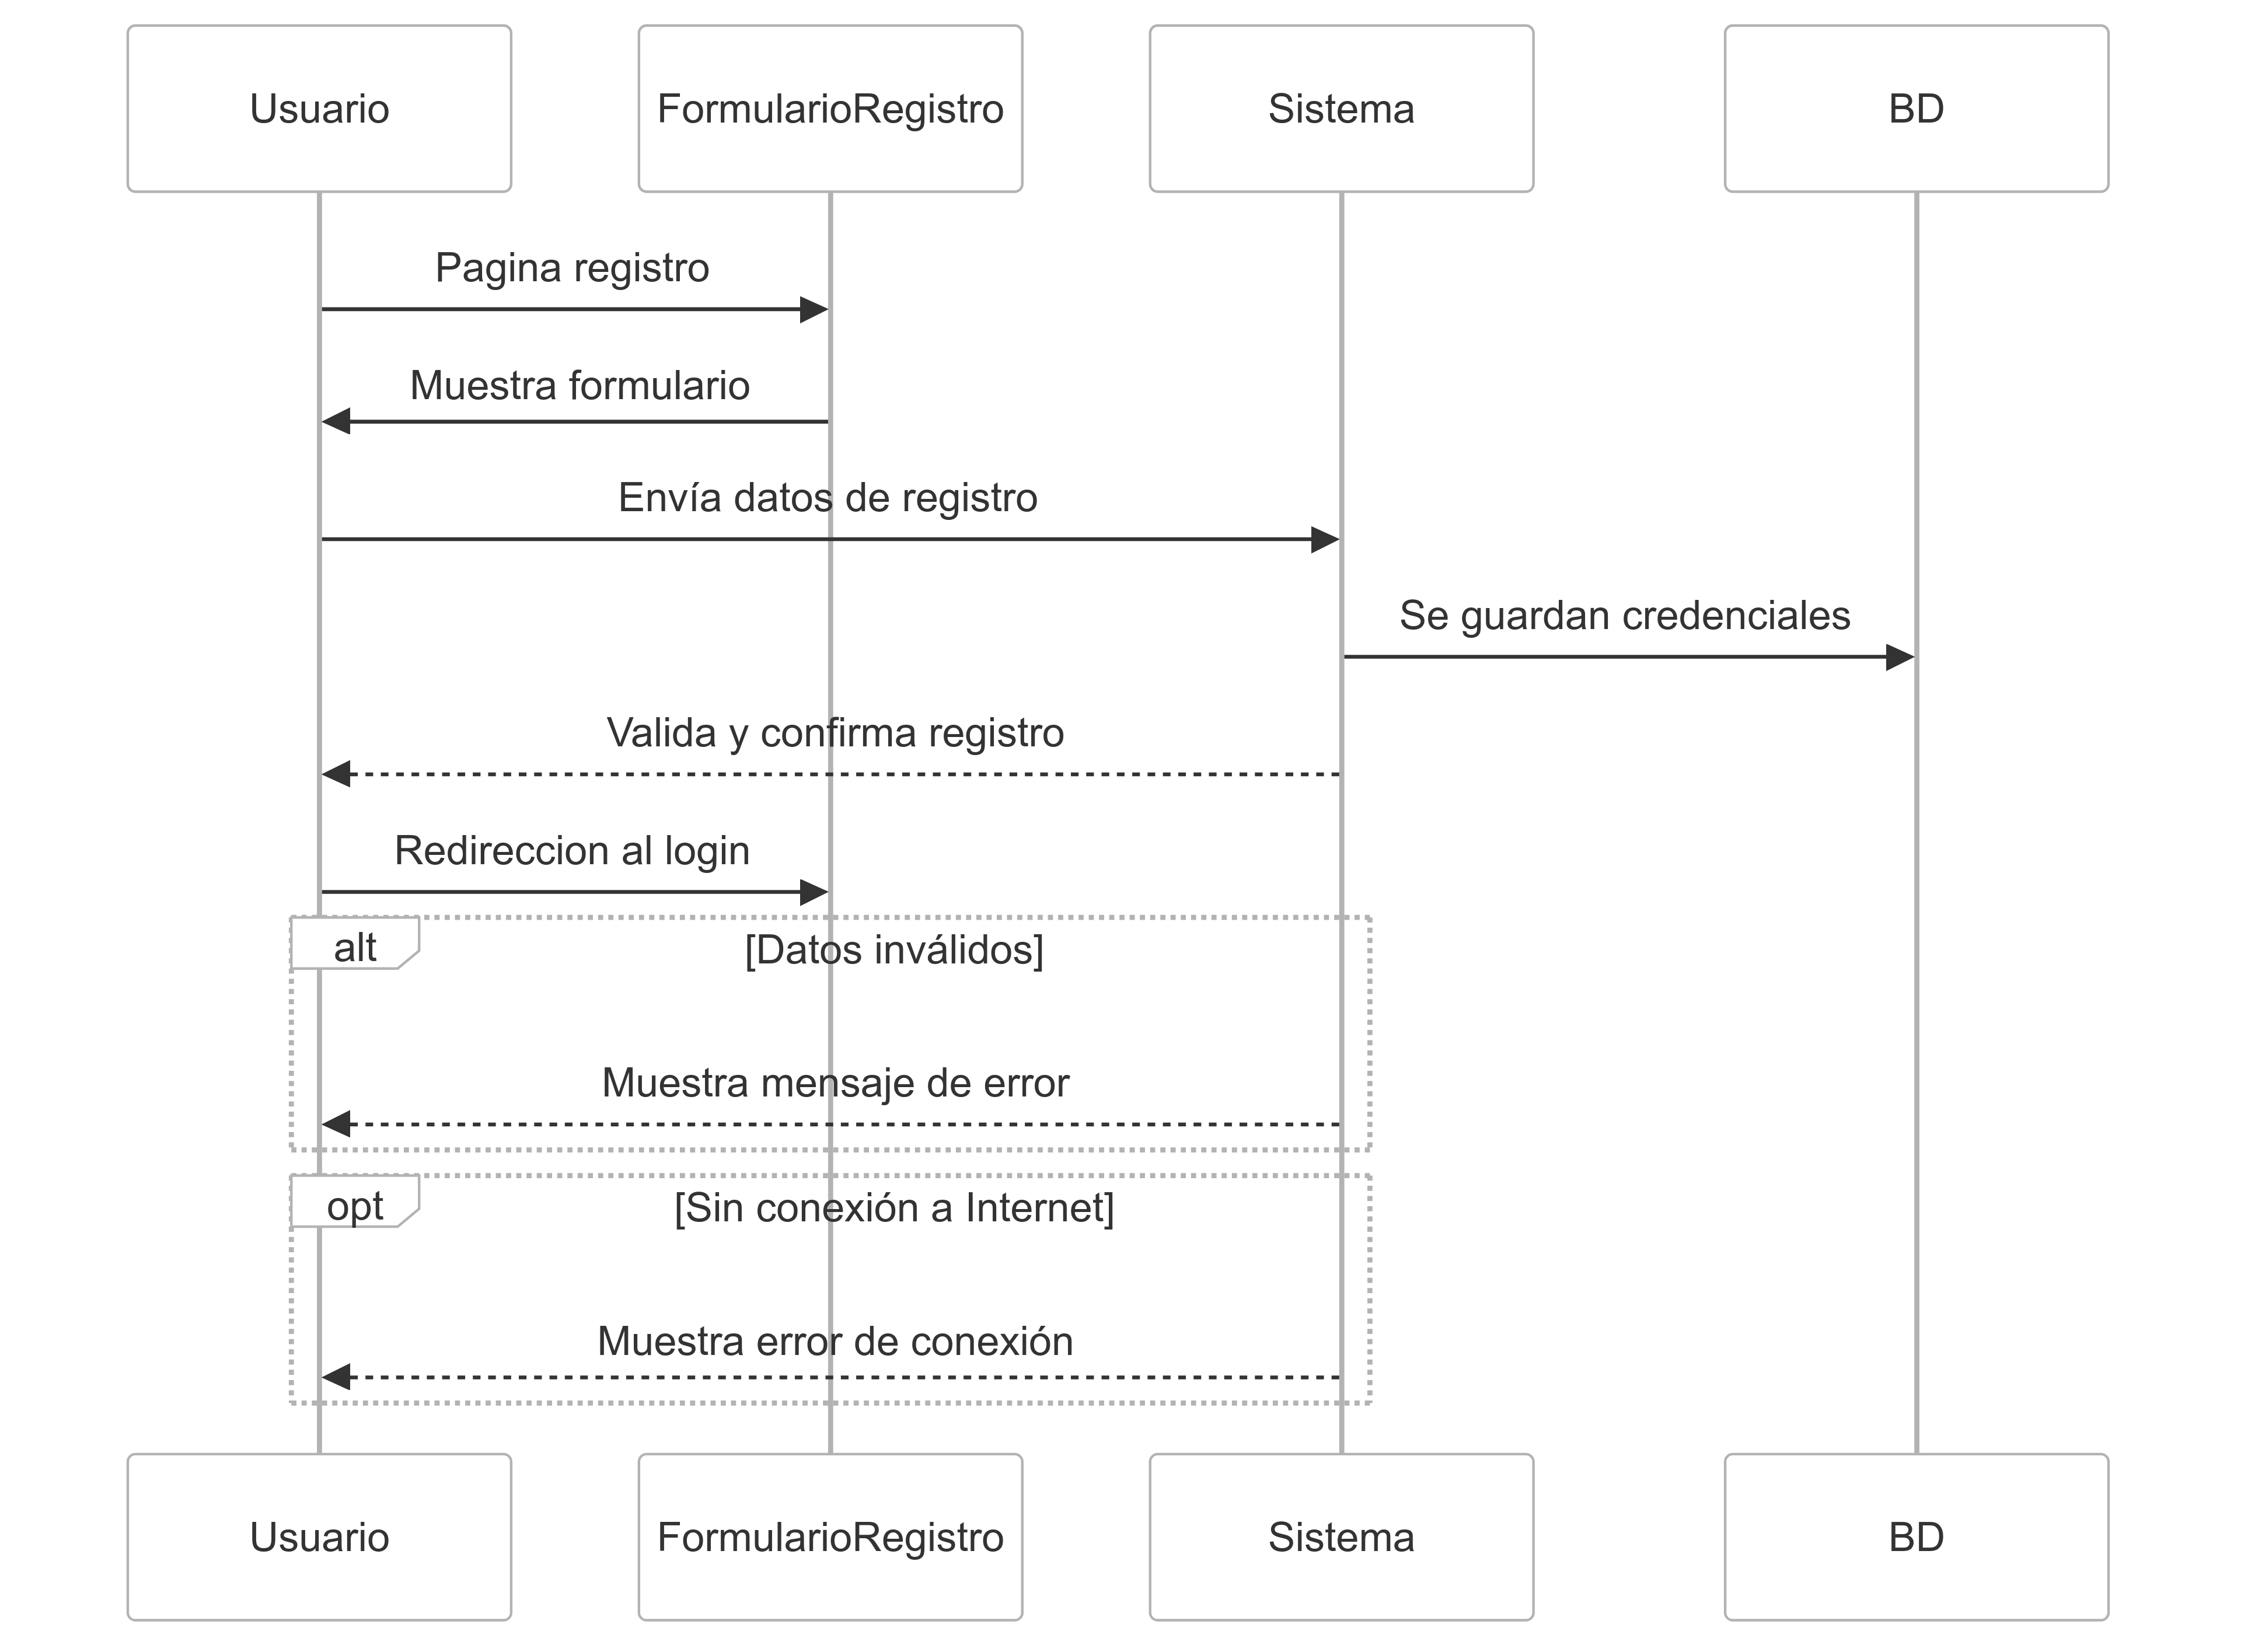
\includegraphics[width=0.5\textwidth]{img/cu1.png} % Adjust width as needed
    \caption{CU1: Registro}
    \label{fig: 1}
\end{figure} 

\begin{figure}[h]
    \centering
    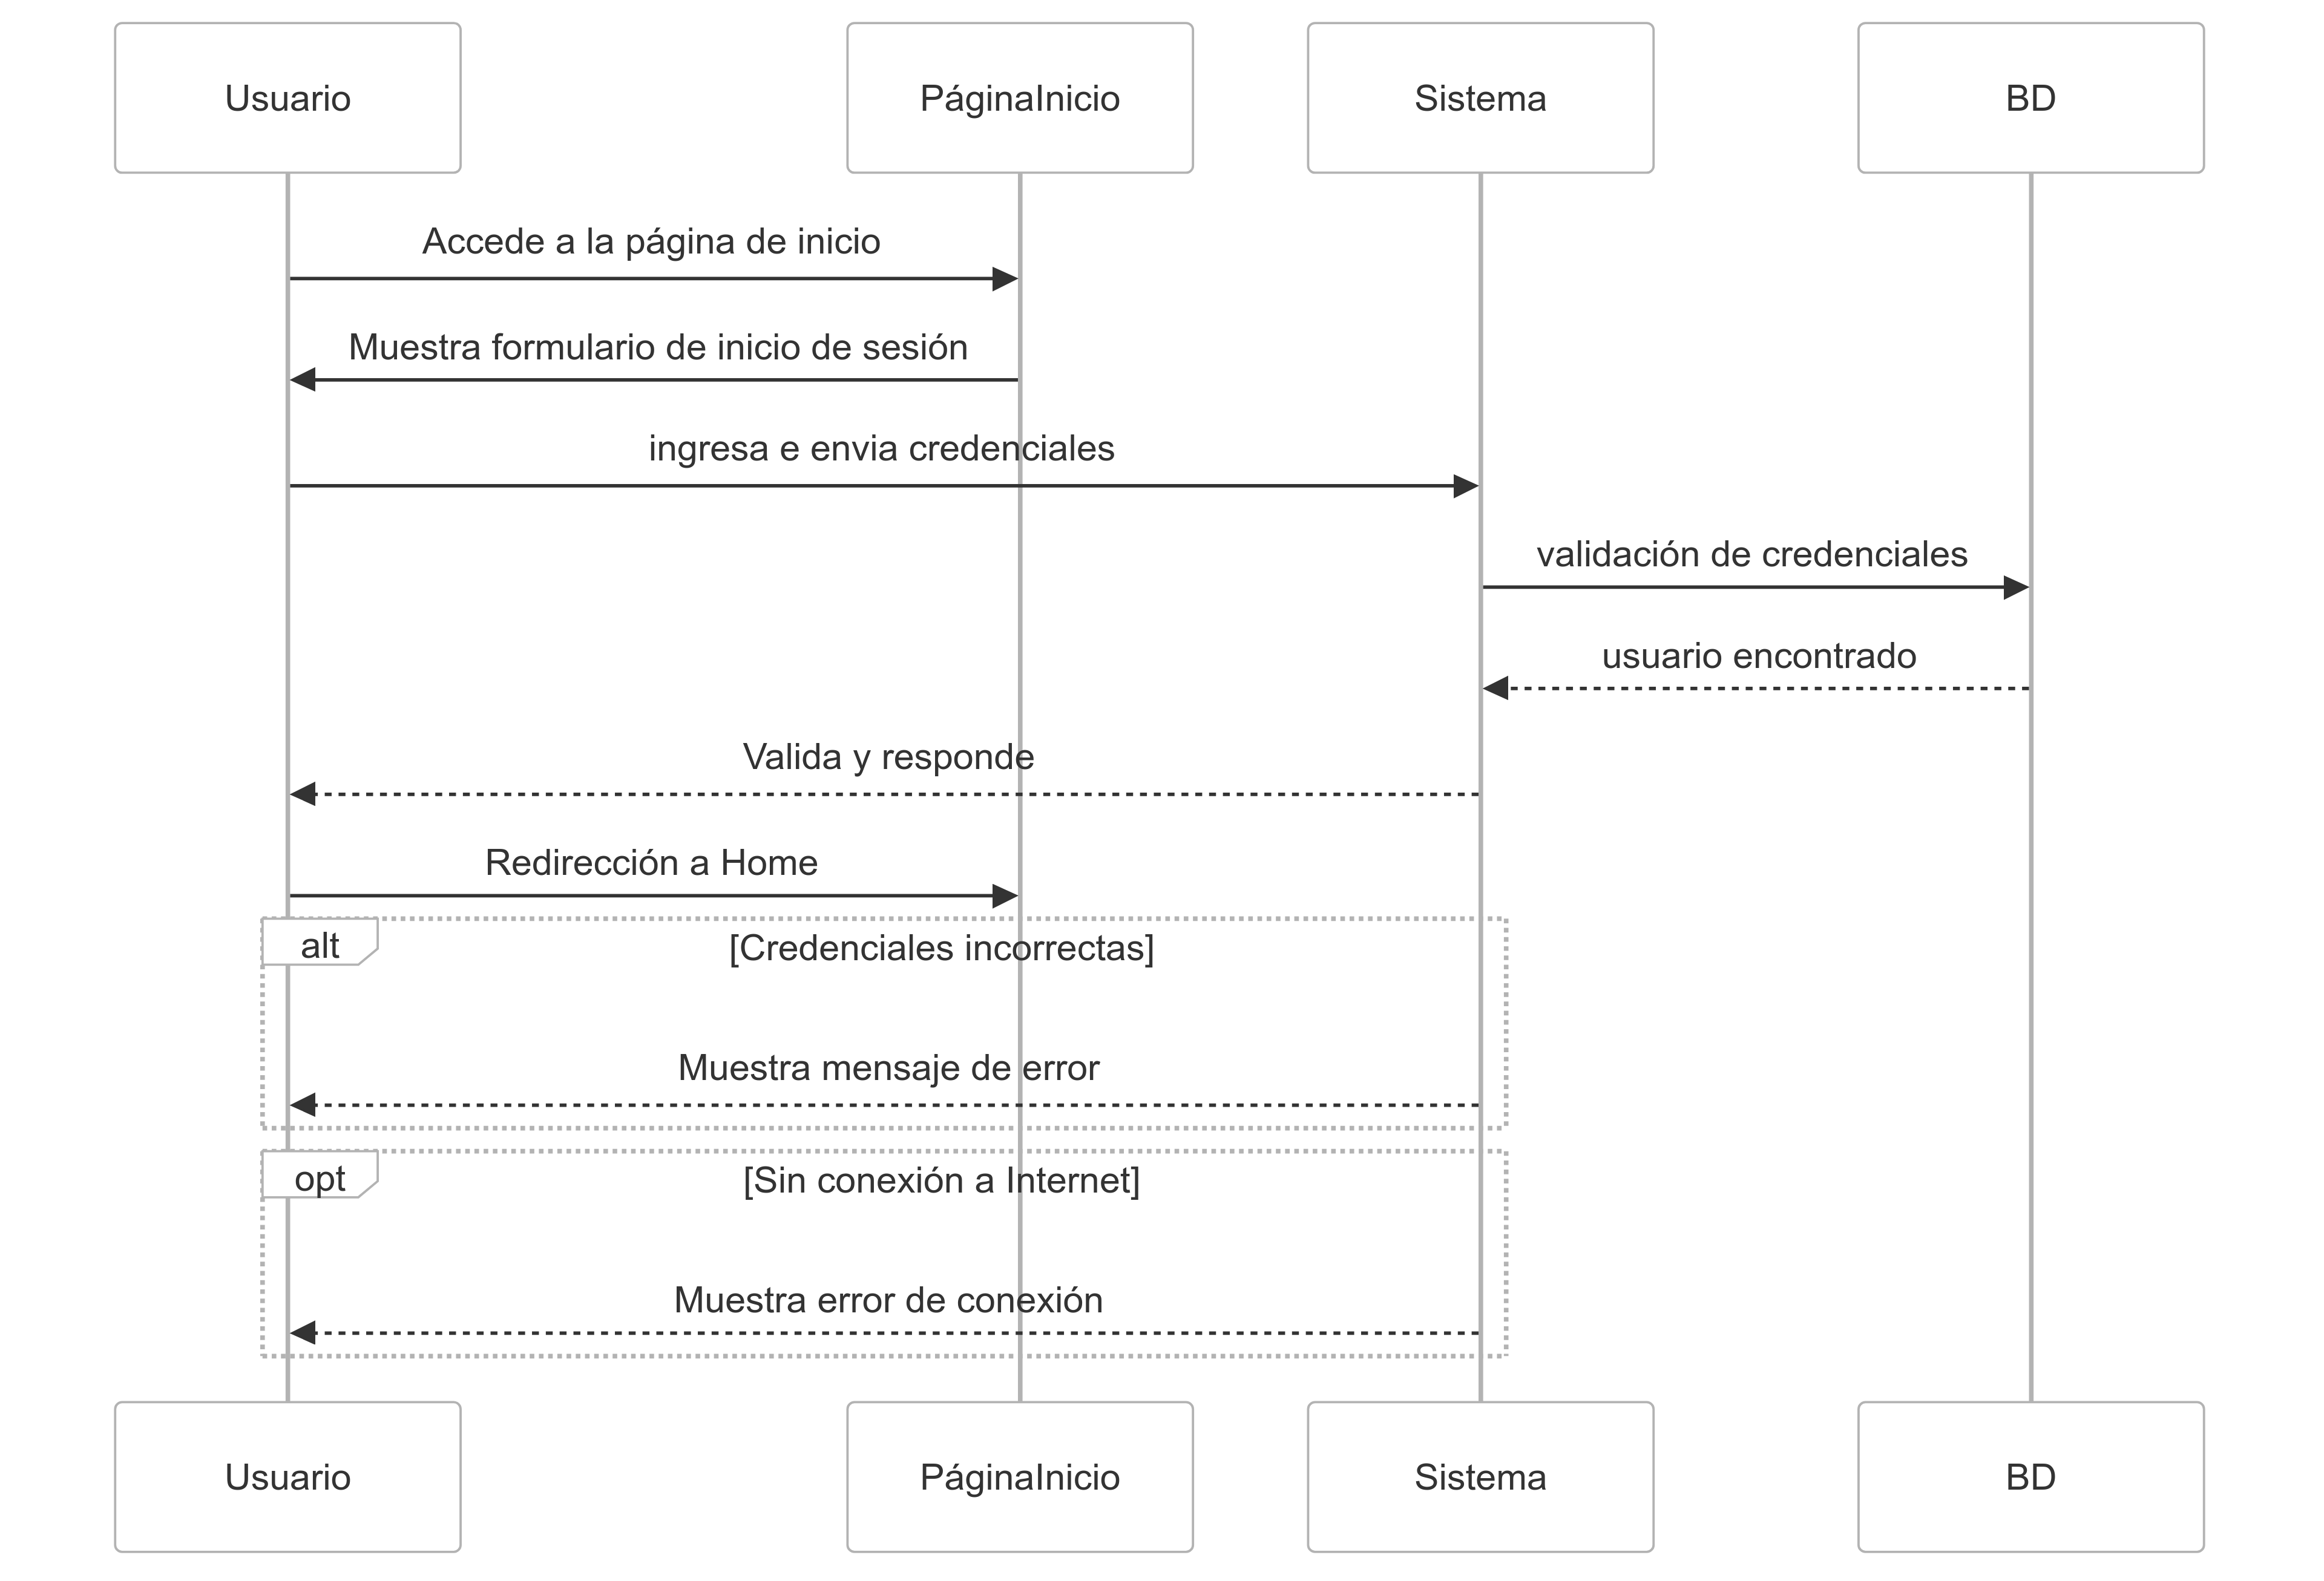
\includegraphics[width=0.5\textwidth]{img/cu2.png} % Adjust width as needed
    \caption{CU2: Inicio de Sesión}
    \label{fig: 1}
\end{figure}

\begin{figure}[h]
    \centering
    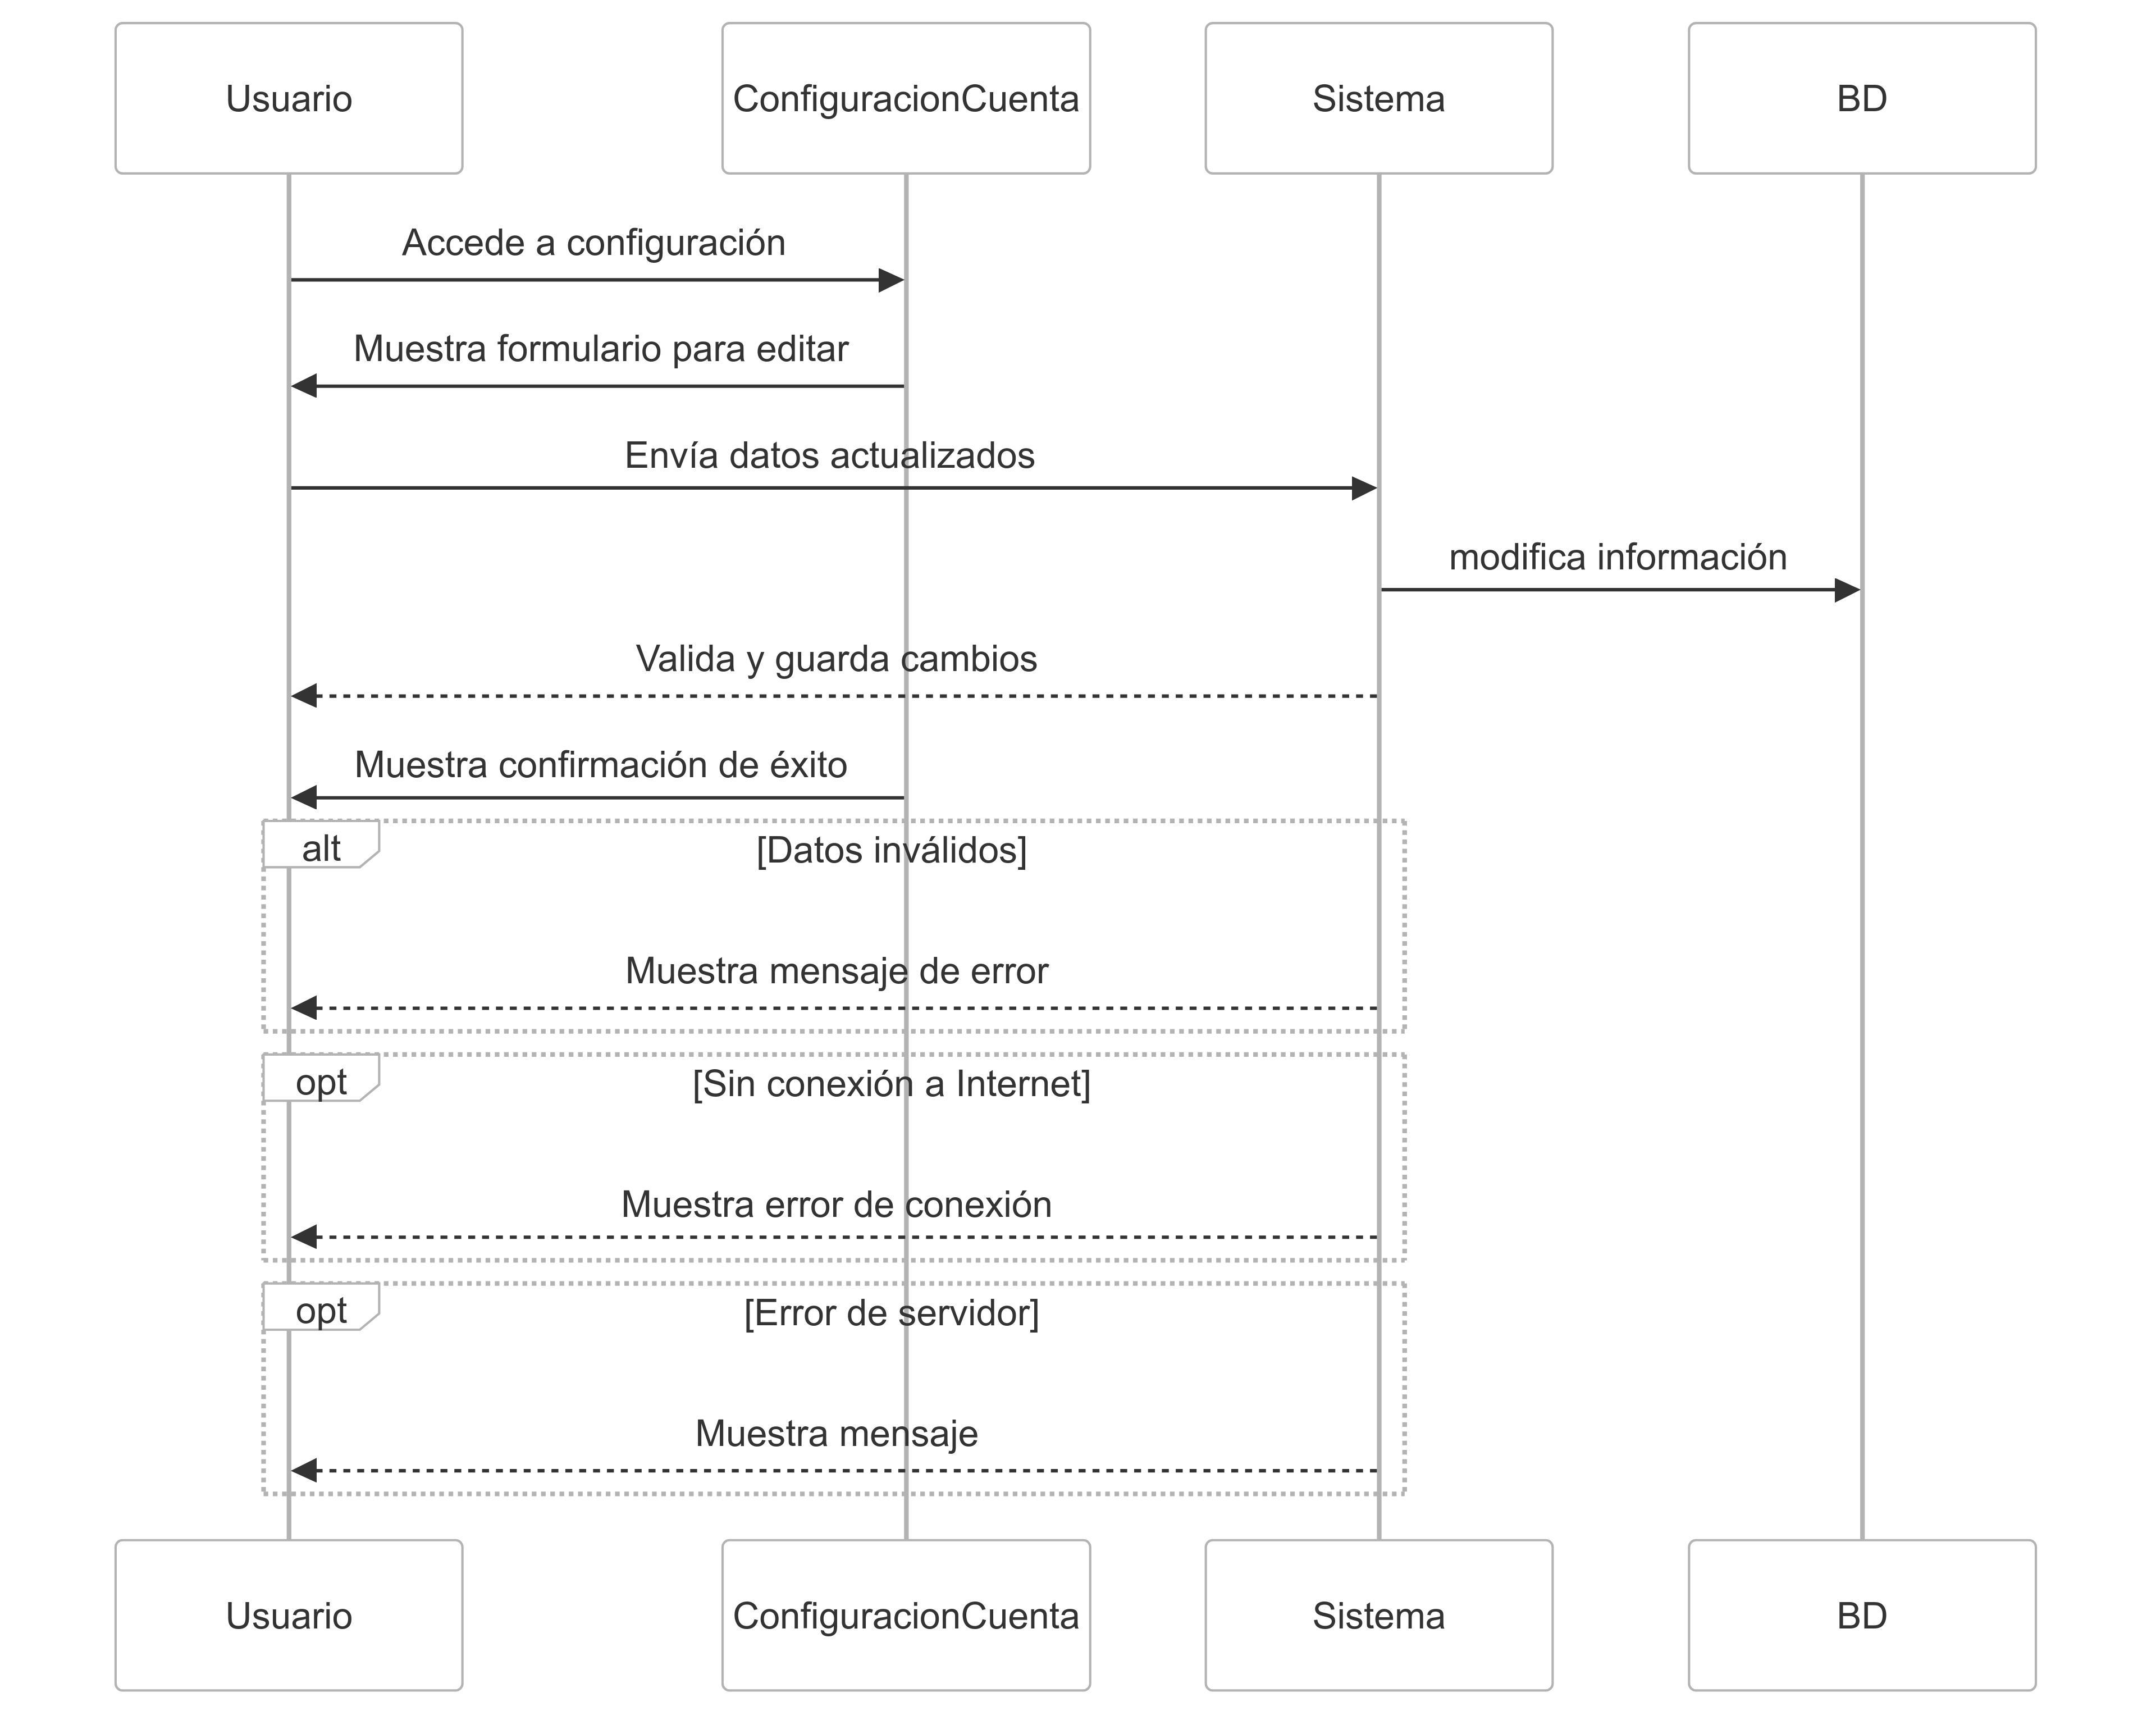
\includegraphics[width=0.5\textwidth]{img/cu3.png} % Adjust width as needed
    \caption{CU3: Editar datos}
    \label{fig: 1}
\end{figure}






\subsection{Requisitos de Hardware y Software}
\subsection{Hardware}
\begin{itemize}
    \item Servidor con al menos 8 GB de RAM y procesador Intel® Core™ i5-6300U, o alguno más potente. Para tener buena velocidad y rendimiento.
    \item Sistema con almacenamiento SSD o HDD para alojar a la base de datos. Esto para tener más flexibilidad.
\end{itemize}

\subsection{Software}
\begin{itemize}
    \item \textbf{Lenguajes de programación:} La implementación se realizará mediante Kotlin debido a que permite que la escritura del código sea más intuitiva conservando las ventajas de Java.
    \item \textbf{Base de datos:} Se usará PostgreSQL debido a que es la herramienta que conoce mayormente el equipo de desarrollo.
    \item \textbf{Framework web:} Se utilizará Spring Boot debido a su facilidad de uso y su extensa comunidad que deriva en un mayor soporte. Además, se hará uso de React.
\end{itemize}


\subsection{Instalación y Configuración}


Este proyecto fue generado utilizando **Angular**, con [Angular CLI](https://github.com/angular/angular-cli) versión 19.2.1.

Para ejecutar el proyecto en un entorno local, sigue estos pasos:

\begin{itemize}
    \item Clonar el repositorio del backend 
    \begin{verbatim}
        git clone https://github.com/ingenieria-software-7009-2025-2/mojarra-Gerreidae-api
    \end{verbatim}
    \item Ejecutar la aplicación MojarraGerreidaeApiApplication.kt ubicada en el repositorio mojarra-gerreidae-api    
    \item Clonar el repositorio del frontend
    \begin{verbatim}
        git clone https://github.com/ingenieria-software-7009-2025-2/mojarra-Gerreidae-frontend.git
        cd mojarra-Gerreidae-frontend
    \end{verbatim}
    \item Instalar dependencias
    \begin{verbatim}
        npm install
    \end{verbatim}
    \item Iniciar el servidor de desarrollo
    \begin{verbatim}
        ng serve
    \end{verbatim}
    \item Abrir la aplicación en el navegador en
    \begin{verbatim}
        http://localhost:4200/
    \end{verbatim}
\end{itemize}  

La aplicación se recargará automáticamente cuando modifiques los archivos fuente.

\textbf{Servidor de desarrollo
}
Para iniciar el servidor de desarrollo, usa:

\begin{verbatim}
    ng serve
\end{verbatim}


\textbf{Generación de código}

Para generar un nuevo componente, usa:

\begin{verbatim}
    ng generate component nombre-del-componente
\end{verbatim}

\textbf{Construcción del proyecto}

Para compilar el proyecto, usa:

\begin{verbatim}
    ng build
\end{verbatim}

Esto generará los archivos compilados en la carpeta `dist/`. De forma predeterminada, la compilación para producción optimiza la aplicación para mejorar el rendimiento.

\textbf{Ejecutar pruebas unitarias}

Para ejecutar las pruebas unitarias con [Karma](https://karma-runner.github.io), usa:

\begin{verbatim}
    ng test
\end{verbatim}

\textbf{Pruebas end-to-end}

Para ejecutar pruebas end-to-end:

\begin{verbatim}
    ng e2e
\end{verbatim}

Angular CLI no incluye un framework de pruebas e2e por defecto, puedes agregar un paquete que lo implemente.

\textbf{Recursos adicionales}

Para más información sobre Angular CLI y su documentación oficial, visita la página de [Angular CLI Overview and Command Reference](https://angular.dev/tools/cli).


\subsection{Documentación API}
Para acceder a la documentación de la API generada por Swagger es necesario: 

\begin{itemize}
    \item Ejecutar la aplicación MojarraGerreidaeApiApplication.kt ubicada en el repositorio mojarra-gerreidae-api
    \item Abrir la aplicación en el navegador en el directorio
    \begin{verbatim}
        http://localhost:8080/swagger-ui/index.html#/
    \end{verbatim}
    
\end{itemize}

\subsection{Consideraciones finales}
Este documento engloba el análisis de requerimientos de nuestro sistema de gestión de incidentes urbanos.

Debido a que se está usando el modelo incremental, nos reservamos el derecho de modificar los requerimientos posteriormente. Aunque claramente sin afectar gravemente la aplicación y las posibles implementaciones ya hechas durante alguna iteración.

Cualquier cambio debe ser aprobado por los interesados.


\end{document}

%%%%%%%%%%%%%%%%%%%%%%%%%%%%%%%%%%%%%%%%

% Copyright Remarks:
%--------------------

% Copyright holder: Vebjørn S. Førde, copyright: CC BY 4.0
% Note: The author of this template is also the copyright holder.

% Below is an explanation of the CC BY 4.0. Additional statements/ 
% clarifications made by the author/copyright holder are marked with *.

% YOU ARE FREE TO:
% Share — copy and redistribute the material in any medium or format
% Adapt — remix, transform, and build upon the material
% for any purpose, even commercially.

% UNDER THE FOLLOWING TERMS:
% Attribution* — You must give appropriate credit, provide a link to the license,
% and indicate if changes were made. You may do so in any reasonable manner, but 
% not in any way that suggests the licensor endorses you or your use.

% *Note: 
% Attribution NOT NEEDED for: 
%       - PDF distibution (like sharing your PDF document)
%       - Use of (dummy)text and images provided in the template (obviously)
%       - Distributing parts of the template, and not the template as a whole
% I am not really concerned with being given credit. As long as you do not 
% claim to have made the template yourself in distributing it further, I have
% no complaints.

% No additional restrictions — You may not apply legal terms or technological 
% measures that legally restrict others from doing anything the license permits.

% NOTICES:
% No warranties are given.

% Disclaimer* (added by copyright holder):
% THE SOFTWARE IS PROVIDED "AS IS", WITHOUT WARRANTY OF ANY KIND, EXPRESS OR
% IMPLIED, INCLUDING BUT NOT LIMITED TO THE WARRANTIES OF MERCHANTABILITY,
% FITNESS FOR A PARTICULAR PURPOSE AND NONINFRINGEMENT. IN NO EVENT SHALL THE
% AUTHORS OR COPYRIGHT HOLDERS BE LIABLE FOR ANY CLAIM, DAMAGES OR OTHER
% LIABILITY, WHETHER IN AN ACTION OF CONTRACT, TORT OR OTHERWISE, ARISING FROM,
% OUT OF OR IN CONNECTION WITH THE SOFTWARE OR THE USE OR OTHER DEALINGS IN THE
% SOFTWARE.

% Read more about CC BY 4.0:
% https://creativecommons.org/licenses/by/4.0/
